\documentclass[../competing_bandits_with_appendix.tex]{subfiles}
\begin{document}
\subsection{Competition vs. Better Algorithms}\label{sec:competition}

% latex table generated in R 3.4.0 by xtable 1.8-2 package
% Thu Aug 16 13:13:01 2018
\begin{table*}[t]
\centering
\begin{adjustbox}{width=\textwidth,center}
\begin{tabular}{|c|c|c|c||c|c|c||c|c|c|}
  \hline
  & \multicolumn{3}{c||}{Heavy-Tail}
  & \multicolumn{3}{c|}{Needle-in-Haystack} 
  & \multicolumn{3}{c|}{Uniform}\\
  \hline
  & $T_0$ = 20 & $T_0$ = 250 & $T_0$ = 500
   & $T_0$ = 20 & $T_0$ = 250 & $T_0$ = 500
  & $T_0$ = 20 & $T_0$ = 250 & $T_0$ = 500 \\
  \hline
\TS vs \DG
  & \textbf{0.31} $\pm$0.03
  & \textbf{0.72} $\pm$0.02
  & \textbf{0.75} $\pm$0.02
  %%
  & \textbf{0.68} $\pm$0.03
  & \textbf{0.62} $\pm$0.03
  & \textbf{0.65} $\pm$0.03 
  %%
  & \makecell{\textbf{0.44} $\pm$0.03} 
 & \makecell{\textbf{0.52} $\pm$0.02} 
 & \makecell{\textbf{0.58} $\pm$0.02} \\
\hline
  $\TS$ vs $\DEG$  
  & \textbf{0.3} $\pm$0.03
  & \textbf{0.89} $\pm$0.01 
  & \textbf{0.9} $\pm$0.01
  %%
  & \textbf{0.6} $\pm$0.03
  & \textbf{0.52} $\pm$0.03
  & \textbf{0.55} $\pm$0.02 
  %%
 & \makecell{\textbf{0.41} $\pm$0.03} 
 & \makecell{\textbf{0.47} $\pm$0.02} 
 & \makecell{\textbf{0.55} $\pm$0.02} \\ \hline
  $\DG$ vs $\DEG$
  & \textbf{0.63} $\pm$0.03 
  & \textbf{0.6} $\pm$0.02
  & \textbf{0.56} $\pm$0.03
  %%
  & \textbf{0.42} $\pm$0.03
  & \textbf{0.41} $\pm$0.03
  & \textbf{0.39} $\pm$0.02
  %%
   & \makecell{\textbf{0.5} $\pm$0.03} 
 & \makecell{\textbf{0.46} $\pm$0.02} 
 & \makecell{\textbf{0.45} $\pm$0.02} \\ \hline
\end{tabular}
\end{adjustbox}
\caption{\footnotesize {\bf Simultaneous Entry, Market Share}. Each cell describes a game between two algorithms, call them Alg1 vs. Alg2, for a particular value of the warm start $T_0$. Each cell contains the market share of Alg 1: the average (in bold) and the 95\% confidence band.
%For example, the cell in the top left indicates that TS gets on average 64\% of the market when played against DG.
 The time horizon is $T=2000$.}
\label{fig:market_share}
\end{table*}



\begin{table*}[t]
\centering
\begin{adjustbox}{width=\textwidth,center}
\begin{tabular}{|c|c|c|c||c|c|c||c|c|c|}
  \hline
  & \multicolumn{3}{c||}{Heavy-Tail}
  & \multicolumn{3}{c|}{Needle-in-Haystack} 
  & \multicolumn{3}{c|}{Uniform}\\
  \hline
  & $T_0$ = 20 & $T_0$ = 250 & $T_0$ = 500
   & $T_0$ = 20 & $T_0$ = 250 & $T_0$ = 500
  & $T_0$ = 20 & $T_0$ = 250 & $T_0$ = 500 \\
  \hline
\TS vs \DG
  & 68 (0)  & 560 (8.5)  & 610 (86.5)
  %%
 & 180 (30)  & 380 (0)  & 550 (6.5)
  %%
  &  260 (0)  
  &  780 (676.5)  
  &  880 (897.5) \\
\hline
  $\TS$ vs $\DEG$  
 & 37 (0)  & 430 (0)  & 540 (105)
  %%
 & 150 (10)  & 460 (25)  & 780 (705)
  %%
 & 230 (0)  & 830 (772)  & 980 (1038) \\ \hline
  $\DG$ vs $\DEG$
 & 340 (110)  & 640 (393)  & 670 (425) 
  %%
  & 410 (8.5)  & 760 (666)  & 740 (646)
  %%
  & 530 (101)  & 990 (1058)  & 1000 (1059) \\ \hline
\end{tabular}
\end{adjustbox}
\caption{\footnotesize {\bf Simultaneous Entry, \Eeog}. Each cell describes a game between two algorithms, call them Alg1 vs. Alg2, for a particular value of the warm start $T_0$. Each cell specifies the ``effective end of game" (\Eeog): the average and the median (in brackets).
%For example, the cell in the top left indicates that TS gets on average 64\% of the market when played against DG. 
The time horizon is $T=2000$.}
\label{fig:eog}
\end{table*}

\normalsize
Our main experiments are with the duopoly game defined in Section~\ref{sec:model}. As the ``intensity of competition" varies from  monopoly to ``incumbent" to simultaneous entry duopoly to ``late entrant", we find a stylized inverted-U relationship \asedit{as in Section~\ref{sec:theory-welfare}}. More formally, we look for equilibria in the duopoly game, where each firm's choices are limited to \DynamicGreedy, \DynamicEpsGreedy and \Thompson. We do this for each ``intensity level" and each MAB instance, and look for findings that are consistent across MAB instances. For cleaner results, we break ties towards less advanced algorithms (as they tend to have lower adoption costs, see \cite{DS-arxiv}). \DynamicGreedy is trivially the dominant strategy under monopoly.

%(1) Permanent monopoly - indifferent between all algorithms but break indifference towards DG cause of deployment costs
%(2) Temporary monopoly - TS is the dominant strategy for the incumbent
%(3) Permanent duopoly -
%   (a) Under NIH, TS is dominant
%   (b) Under Heavy Tail, DG is weakly dominant
%   (c) Under Uniform, DG "beats" TS, but DEG "beats" TS by more than DG and DEG vs DG leads to ~50% market share (it's slightly in favor of DG but 50/50 is within the confidence band). If we break indifference towards DG cause of deployment costs, then we have that the unique PSNE is (DG, DG). If we don't add the indifference breaking, then we have four PSNE, (DG, DEG), (DEG, DG), (DG, DG), (DEG, DEG)


\xhdr{Simultaneous entry.}
The basic scenario is when both firms are competing from round $1$. A crucial distinction is whether an MAB instance is exploration-disadvantaged:

\begin{finding}\label{find:duopoly}
\textit{Under simultaneous entry:
\begin{itemize}
\item[(a)] (\DynamicGreedy,\DynamicGreedy) is the unique pure-strategy Nash equilibrium for exploration-disadvantaged MAB instances with a sufficiently small ``warm start".
\item[(b)] This is not necessarily the case for MAB instances that are not exploration-disadvantaged. In particular, \Thompson is a weakly dominant strategy for Needle-in-Haystack.
\end{itemize}
}
\end{finding}


%\begin{finding}
%\textit{For sufficiently low warm start under the instances that are exploration-disadvantaged, the unique incentivized strategies in the competition game are:\footnote{The uniqueness comes from the fact that we break indifferences towards easier to deploy algorithms}
%\begin{center}
%\textbf{Permanent Monopoly} - $\DG$ \\
%\textbf{Temporary Monopoly} (incumbent)- $\TS$ \\
%\textbf{Permanent Duopoly} - $(\DG, \DG)$ \\
%\end{center}
%The conditions on $\TS$ being dominant under the temporary monopoly are that the incumbent is a temporary monopoly for sufficiently many periods.}
%\end{finding}

%\xhdr{Permanent Monopoly.} Since there is only a single firm in the
%market for the entire period, the firm can take the entire market
%regardless of what algorithm it deploys. \swedit{Since we assume that exploration algorithms ($\DEG$ and $\TS$) would incur deployment cost and firms break indifferences towards easier to deploy algorithms}, the firm would choose to deploy $\DG$.

We investigate the firms' market shares when they choose different algorithms (otherwise, by symmetry both firms get half of the agents). We report the market shares for \gaedit{each instance in} Table~\ref{fig:market_share}. We find that $\DG$ is a weakly dominant strategy for the Heavy-Tail and Uniform instances, as long as $T_0$ is sufficiently small. However, \Thompson is a weakly dominant strategy for the Needle-in-Haystack instance. We find that for a sufficiently small $T_0$, \DynamicGreedy yields more than half the market against \Thompson,  but achieves similar market share vs. \DynamicGreedy and \DynamicEpsGreedy. By our tie-breaking rule, (\DynamicGreedy,\DynamicGreedy) is the only pure-strategy equilibrium.


\OMIT{This establishes our claim that $\DG$ is the incentivized algorithm.\footnote{We defer the table for uniform instances to the appendix. Summarizing the results, we see that, for low warm start, \DG yields more than half the market against \TS but is indifferent between \DG and \DEG. Since we break indifference towards easier to deploy algorithms, we also find that \DG is the incentivized algorithm in equilibrium}}

We attribute the prevalence of \DynamicGreedy on exploration-disadvantaged MAB instances to its prevalence on the initial ``exploration disadvantage period", as described in Section~\ref{sec:isolation}. Increasing the warm start length $T_0$ makes this period shorter: indeed, considering the relative reputation trajectory in Figure~\ref{relative_rep_plots} (left), increasing $T_0$ effectively shifts the starting time point to the right. This is why it helps \DynamicGreedy if $T_0$ is small.


\OMIT{
The reason we see that $\DynamicGreedy$ is incentivized under the Heavy Tail and Uniform instances but that $\Thompson$ is weakly dominant under Needle In Haystack is precisely due to the fact that the purposeful exploration engaged by $\Thompson$ in the early rounds puts it in a disadvantage in the former case but not in the latter. Looking at the relative reputation plots in Figure \ref{relative_rep_plots}, we can interpret fixing a warm start $T_0$ as fixing the starting point on the relative reputation plots. The proportion of first rounds in the competition game that will go to a firm playing alg $A$ over a firm playing alg $B$ will correspond to the relative reputation proportion at time $T_0$. As a result, we see that for warm start $T_0 = 20$ on the exploration-disadvantaged instances, $\DynamicGreedy$ will win the first agent in a larger proportion of the simulations than $\Thompson$. However, on the Needle In Haystack instances, we see that $\Thompson$ wins a larger proportion of the first agents compared to $\DynamicGreedy$.
}

\xhdr{First-Mover.}
We turn our attention to the first-mover scenario. Recall that the incumbent firm enters the market and serves as a monopolist until the entrant firm enters at round $X$. We make $X$ large enough, but still much smaller than the time horizon $T$. We find that the incumbent is incentivized to choose \Thompson, in a strong sense:

\begin{finding}\label{find:temp-monopoly}
\textit{Under first-mover, \Thompson is the dominant strategy for the incumbent. This holds across all MAB instances, if $X$ is large enough.
}
\end{finding}

The simulation results for the Heavy-Tail MAB instance are reported in Table~\ref{tab:ht-incum}, for a particular $X=200$. We see that \Thompson is a dominant strategy for the incumbent. Similar tables for the other MAB instances and other values of $X$ are reported in the supplement, with the same conclusion.

\begin{table}[H]
\centering
\begin{tabular}{|c|c|c|c|}
\hline
   & $\TS$  & $\DEG$  & $\DG$ \\ \hline
$\TS$
    & \makecell{\textbf{0.003}$\pm$0.003}
    & \makecell{\textbf{0.083}$\pm$0.02}
    & \makecell{\textbf{0.17}$\pm$0.02} \\\hline
$\DEG$
    & \makecell{\textbf{0.045}$\pm$0.01}
    & \makecell{\textbf{0.25}$\pm$0.02}
    & \makecell{\textbf{0.23}$\pm$0.02} \\\hline
$\DG$
    & \makecell{\textbf{0.12}$\pm$0.02}
    & \makecell{\textbf{0.36}$\pm$0.03}
    & \makecell{\textbf{0.3}$\pm$0.02} \\\hline
\end{tabular}
\caption{\footnotesize Market share of row player (entrant), 200 round head-start, Heavy-Tail Instance}
%\caption{{\bf Temporary monopoly}, with $X=200$ (and $T_0=20$), for the Heavy-Tail MAB instance. Each cell describes the duopoly game between the entrant's algorithm (the row) and the incumbent's algorithm (the column). The cell specifies the entrant's market share (fraction of rounds in which it was chosen) for the rounds in which he was present. We give the average (in bold) and the 95\% confidence interval. NB: smaller average is better for the incumbent.}
\label{tab:ht-incum}
\end{table}
\OMIT{
\begin{table}[h]
\centering
\caption{Heavy Tail}
\begin{tabular}{|c|c|c|c|}
\hline
   & $\TS$  & $\DEG$  & $\DG$ \\ \hline
$\TS$
    & \makecell{\textbf{0.50, 0.50}}
    & \makecell{\textbf{0.3, 0.7}}
    & \makecell{\textbf{0.29, 0.71}} \\\hline
$\DEG$
    & \makecell{\textbf{0.7, 0.3}}
    & \makecell{\textbf{0.50, 0.50}}
    & \makecell{\textbf{0.38, 0.62}} \\\hline
$\DG$
    & \makecell{\textbf{0.71, 0.29}}
    & \makecell{\textbf{0.62, 0.38}}
    & \makecell{\textbf{0.50, 0.50}} \\\hline
\end{tabular}
\end{table}

\begin{table}[h]
\centering
\caption{Needle In Haystack}
\begin{tabular}{|c|c|c|c|}
\hline
   & $\TS$  & $\DEG$  & $\DG$ \\ \hline
$\TS$
    & \makecell{\textbf{0.50, 0.50}}
    & \makecell{\textbf{0.57, 0.43}}
    & \makecell{\textbf{0.64, 0.36}} \\\hline
$\DEG$
    & \makecell{\textbf{0.43, 0.57}}
    & \makecell{\textbf{0.50, 0.50}}
    & \makecell{\textbf{0.54, 0.46}} \\\hline
$\DG$
    & \makecell{\textbf{0.36, 0.64}}
    & \makecell{\textbf{0.43, 0.57}}
    & \makecell{\textbf{0.50, 0.50}} \\\hline
\end{tabular}
\end{table}
}


\DynamicGreedy is a weakly dominant strategy for the entrant, for Heavy-Tail instance in Table~\ref{tab:ht-incum} and the Uniform instance, but not for the Needle-in-Haystack instance. We attribute this finding to exploration-disadvantaged property of these two MAB instance, for the same reasons as discussed above.

\begin{finding}\label{find:temp-monopoly-entrant}
\textit{Under first-mover, \DynamicGreedy is a weakly dominant strategy for the entrant for exploration-disadvantaged MAB instances.
}
\end{finding}


\tikzstyle{level 1}=[level distance=3.5cm, sibling distance=4.0cm]
\tikzstyle{level 2}=[level distance=3.5cm, sibling distance=2cm]
\tikzstyle{below} = [align=center]

\begin{figure}[t]
\begin{center}
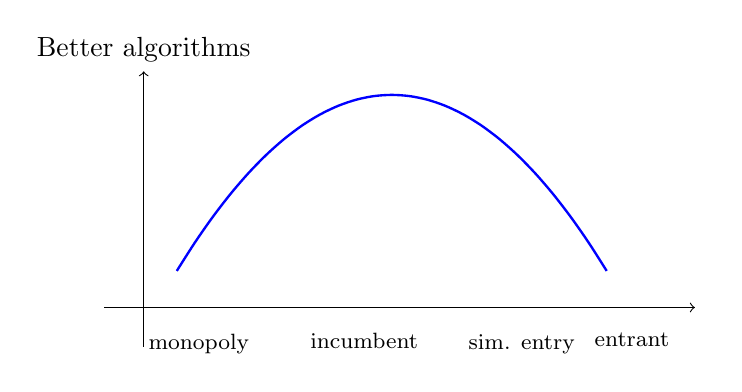
\begin{tikzpicture}
      \draw[->] (-.5,0) -- (7,0) node[right] {};
      \draw[->] (0,-.5) -- (0,3) node[above] {Better algorithms};
      \draw[scale=0.6,domain=0.7:9.8,smooth,variable=\x,blue, line width=0.3mm] plot ({\x},{4.5 - 0.18 * (\x - 5.25)^2});
     \node[below] at (0.7, -0.22) {\footnotesize monopoly};
     \node[below] at (2.8, -0.2) {\footnotesize incumbent};
     \node[below] at (4.8, -0.22) {\footnotesize sim. entry};
     \node[below] at (6.2, -0.2) {\footnotesize entrant};
 \end{tikzpicture}
 \caption{\footnotesize A stylized ``inverted-U relationship" between strength of competition and ``level of innovation".}
\label{fig:inverted-U-expts}
\end{center}
\end{figure}

\xhdr{Inverted-U relationship.}
We interpret our findings through the lens of the inverted-U relationship between the ``intensity of competition" and the ``quality of technology". The lowest level of competition is monopoly, when \DynamicGreedy wins out for the trivial reason of tie-breaking. The highest levels are simultaneous entry and ``late entrant". We see that \DynamicGreedy is incentivized for exploration-disadvantaged MAB instances. In fact, incentives for \DynamicGreedy get stronger when the model transitions from simultaneous entry to ``late entrant".%
\footnote{For the Heavy-Tail instance, \DynamicGreedy goes from a weakly dominant strategy to a strictly dominant one. For the Uniform instance, \DynamicGreedy goes from a Nash equilibrium strategy to a weakly dominant one.}
Finally, the middle level of competition, ``incumbent" in the first-mover regime creates strong incentives for \Thompson. In stylized form, this relationship is captured in Figure~\ref{fig:inverted-U-expts}.%
\footnote{We consider the monopoly scenario for comparison only, without presenting any findings. We just assume that a monopolist chooses
the greedy algorithm, because it is easier to deploy in practice. Implicitly, users have no ``outside option": the service provided is an improvement over not having it (and therefore the monopolist is not incentivized to deploy better learning algorithms). This is plausible with free ad-supported platforms such as Yelp or Google.}


% Transition Duopoly -> LateStart creates stronger incentives for DG.
% In Heavy Tail, DG is strictly dominant (before it was only weakly).
% In Uniform, DG is weakly dominant (before it was only PSNE).

Our intuition for why incumbency creates more incentives for exploration is as follows. During the period in which the incumbent is the only firm in the market, reputation consequences of exploration vanish. Instead, the firm wants to improve its performance as much as possible by the time competition starts. Essentially, the firm only faces a classical explore-exploit trade-off, and is incentivized to choose algorithms that are best at optimizing this trade-off.

\xhdr{Death spiral effect.}
Further, we investigate the ``death spiral" effect mentioned in the Introduction. Restated in terms of our model, the effect is that one firm attracts new customers at a lower rate than the other, and falls behind in terms of performance because the other firm has more customers to learn from, and this gets worse over time until (almost) all new customers go to the other firm. With this intuition in mind, we define  \textit{effective end of game} (\Eeog) for a particular \MRV and realization table, as the last round $t$ such that the agents at this and previous round choose different firms. Indeed, the game, effectively, ends after this round. We interpret low \Eeog as a strong evidence of the ``death spiral" effect. Focusing on the simultaneous entry scenario, we specify the \Eeog values in Table~\ref{fig:eog} (the second line of each cell). We find that the \Eeog values are indeed small:

\begin{finding}
\textit{
Under simultaneous entry, \Eeog values tend to be much smaller than the time horizon $T$.
}
\end{finding}

We also see that the \Eeog values tend to increase as the warm start $T_0$ increases. We conjecture this is because larger $T_0$ tends to be more beneficial for a better algorithm (as it tends to follow a better learning curve). Indeed, we know that the ``effective end of game" in this scenario typically occurs when a better algorithm loses, and helping it delays the loss.


\xhdr{Welfare implications.}
We study the effects of competition on consumer welfare: the total reward collected by the users over time. Rather than welfare directly, we find it more lucid to consider
\emph{market regret}:
\[ \textstyle T\, \max_a \mu(a) - \sum_{t\in [T]} \mu(a_t), \]
where $a_t$ is the arm chosen by agent $t$. This is a standard performance measure in the literature on multi-armed bandits. Note that smaller regret means higher welfare.


\begin{figure}
\centering
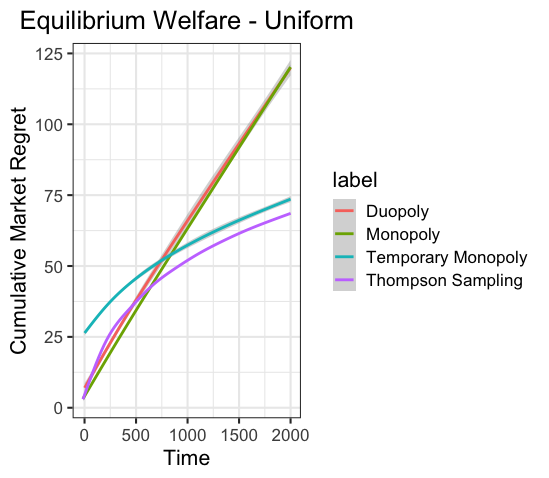
\includegraphics[scale=0.35]{ec19paper/figures/unif_eq_welfare}
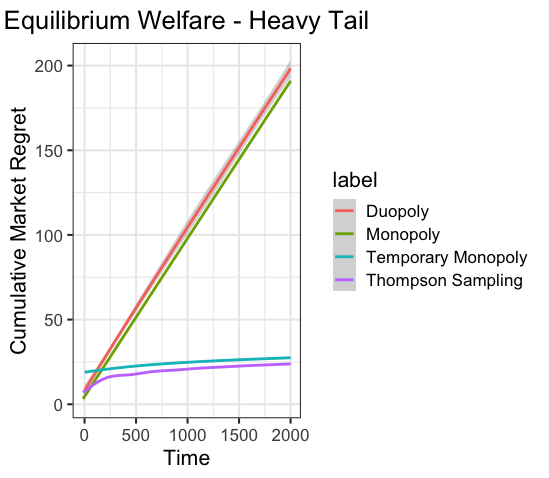
\includegraphics[scale=0.35]{ec19paper/figures/ht_eq_welfare}
\caption{\footnotesize Smoothed welfare plots resulting from equilibrium strategies in the different market structures. Note that welfare at $t = 0$ incorporates the regret incurred during the incumbent and warm start periods. The Thompson Sampling trajectory displays the regret incurred by running Thompson Sampling in isolation on the given instances.}
\label{eq_regret}
\end{figure}

We assume that both firms play their respective equilibrium strategies for the corresponding competition level. As discussed previously, these are:
\begin{OneLiners}
\item \DynamicGreedy in the monopoly,
\item \DynamicGreedy for both firms in simultaneous entry (Finding \ref{find:duopoly}),
\item \Thompson for the incumbent (Finding \ref{find:temp-monopoly}) and \DynamicGreedy for the entrant in first-mover (Finding \ref{find:temp-monopoly-entrant}).
\end{OneLiners}

Figure \ref{eq_regret} displays the market regret (averaged
  over multiple runs) under different levels of competition.
Consumers are \textit{better off} in the first-mover case than in
the simultaneous entry case. Recall that under first-mover, the incumbent is incentivized to play \Thompson. Moreover, we find that the welfare is close to that of having a single firm for all agents and running \Thompson. We also observe that monopoly and simultaneous entry achieve similar welfare.
%with monopoly being marginally better than duopoly.

\begin{finding}\label{find:welfare}
\textit{In equilibrium, consumer welfare is (a) highest under first-mover, (b) similar for monopoly and simultaneous entry.
%monopoly being marginally better leading to marginally better welfare than duopoly.
}
\end{finding}

Finding~\ref{find:welfare}(b) is interesting because, in equilibrium, both firms play \DynamicGreedy in both settings, and one might conjecture that the welfare should increase with the number of firms playing \DynamicGreedy. Indeed, one run of \DynamicGreedy may get stuck on a bad arm. However, two firms independently playing \DynamicGreedy are less likely to get stuck simultaneously. If one firm gets stuck and the other does not, then the latter should attract most agents, leading to improved welfare.
\begin{figure}
\centering
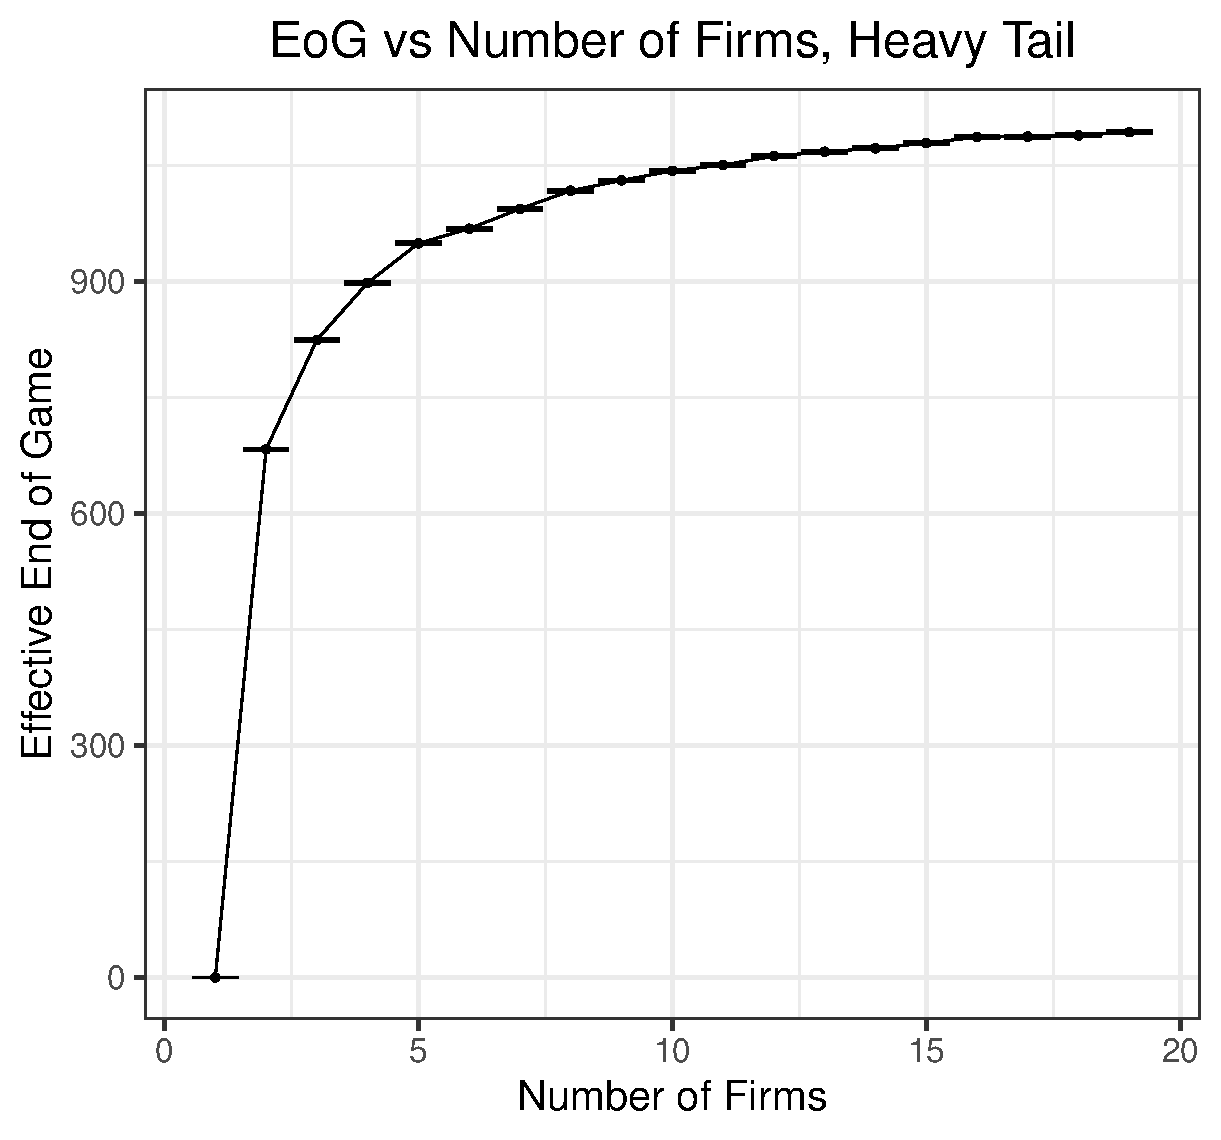
\includegraphics[scale=0.3]{ec19paper/figures/eeog_vs_num_firms_ht}
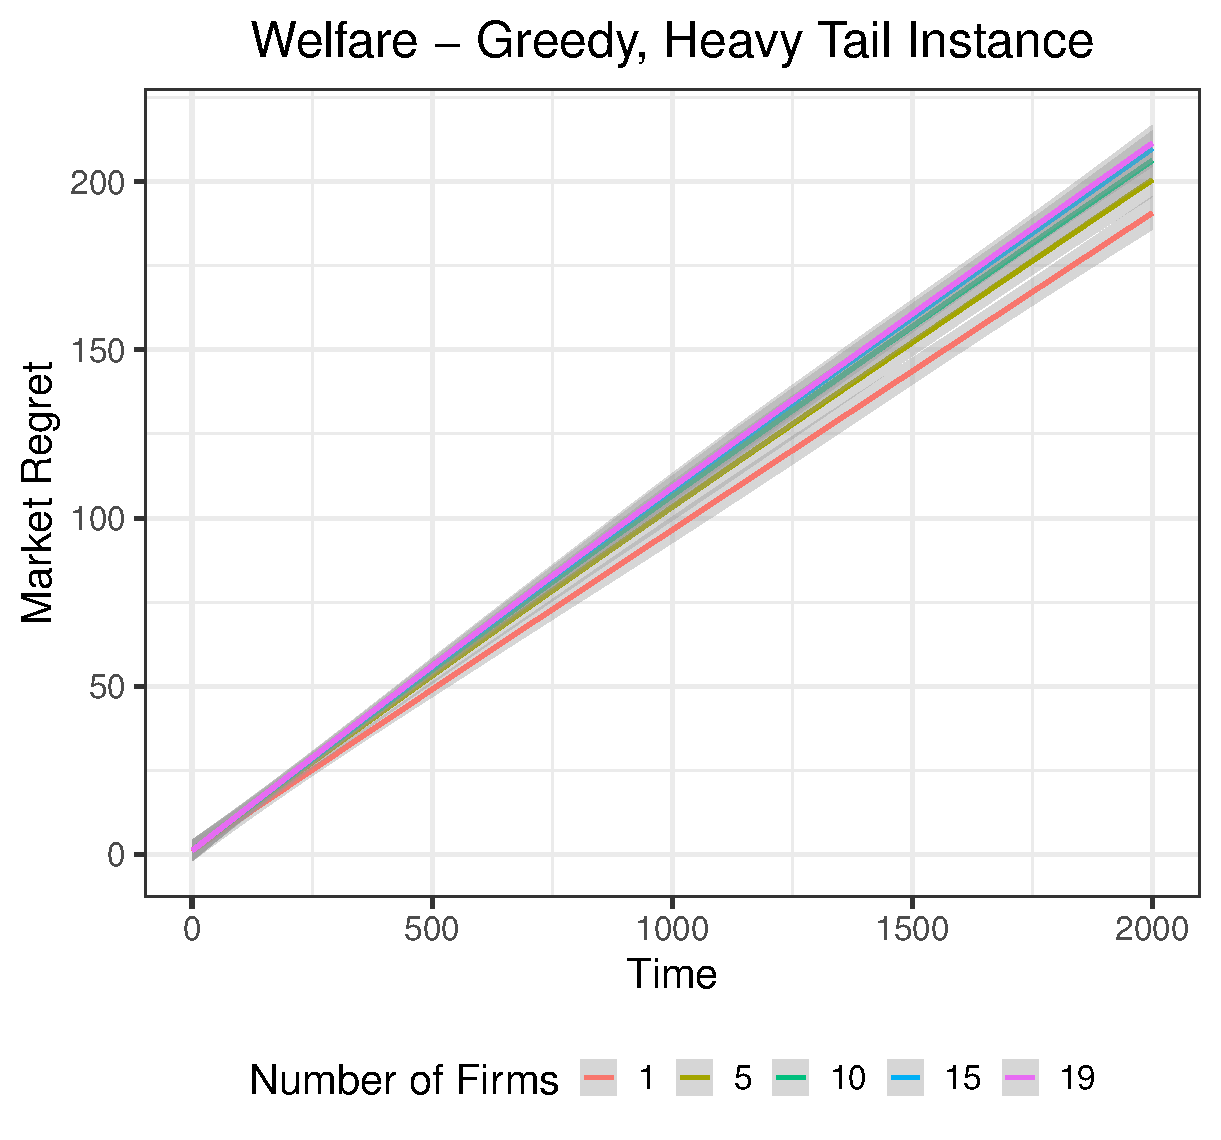
\includegraphics[scale=0.3]{ec19paper/figures/ht_many_firm_welfare}\\
\caption{Average welfare and \Eeog as we increase the number of firms playing \DynamicGreedy}
\label{many_firm_welfare}
\end{figure}

To study this phenomenon further, we go beyond the duopoly setting to more than two firms playing \DynamicGreedy (and starting at the same time). Figure~\ref{many_firm_welfare} reports the average welfare
across these simulations. Welfare not only does not get better, \textit{but is weakly worse} as we increase the number of firms.

\begin{finding}
\textit{When all firms deploy \DynamicGreedy, and start at the same time, welfare is weakly decreasing as the number of firms increases.}
\end{finding}


We track the average \Eeog in each of the
simulations and notice that it \textit{increases} with the number of firms.
This observation also runs counter of the intuition that with more firms running \DynamicGreedy, one of them is more likely to ``get lucky" and take over the market (which would cause \Eeog to \emph{decrease} with the number of firms).

\OMIT{As we increase the number of firms, a single
individual firm gets fewer consumers for learning as consumers switch
between firms more often. Additionally, bad luck with rewards or arm
selection is punished even more harshly as we increase the number of
firms. This further strengthens the intuition from our previous
result, which is that learning may be hard under competition since
exploration and mistakes are punished harshly but are necessary for
learning.}


\end{document}
%%% Local Variables:
%%% mode: latex
%%% TeX-master: "../competing_bandits"
%%% End: 